\documentclass[a4paper]{book}
\usepackage{graphicx}
\title{Fundamentals of Financial Forecasting}
\begin{document}
\chapter{Introduction}
A typical goal in the financial arena is to attempt to predict the future based upon knowledge of the past, in order to make profitable trades.
In this document, we shall look primarily at the analysis of financial timeseries data, in particular the prices of stocks.
For illustrative purposes, most of our examples will be drawn from the analysis of the price history of just a few stocks, as shown
in Figure~\ref{fig:stock-prices}. Of course, in practice one must collect and analyse a large amount of data for a wide variety of stocks, 
in order to obtain more general and robust predictive models.

\chapter{Basic Time-Series Modelling}
\section{One-step Predictive Models}
Consider the stock prices shown in Figure~\ref{fig:stock-prices},
which vary daily over a period of time.
Each sequence of prices for a given stock forms a time-series.
Here let $V(t)$ be the price of a given stock at time $t$. In general,
$V(t)$ represents the time-varying value of any asset. We
consider only the gross, not net, asset value, and hence may assume that $V(t)\ge 0$.
\begin{figure}[hbt]
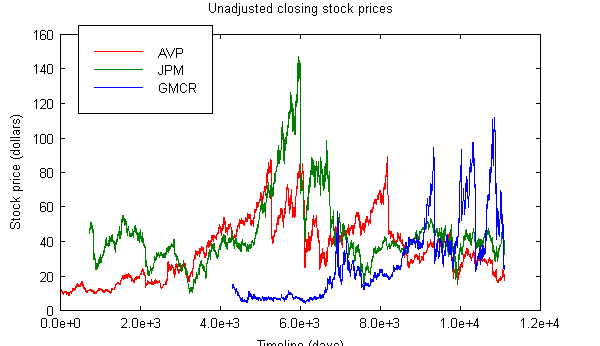
\includegraphics[scale=0.8]{figures/stock-prices-close.png}
\caption{Example data showing the unadjusted closing prices of three different
types of stock.}
\label{fig:stock-prices}
\end{figure}

Although the value $V(t)$ varies continuously with time $t$,
the stock prices shown in Figure~\ref{fig:stock-prices} were in
fact sampled at the close of each day of trading.
Thus, rather than knowing $V(t)$ for all $t$, we only know
a finite set of values $V(t_n)$ at fixed times $t_n=t_0+n\delta t$,
for $n=0,1,\ldots,m$. The interval of time specified by $\delta t$
is known as a {\em bar}. In our example,
1 bar is equivalent to 1 day, and this shall henceforth 
be assumed to be true unless otherwise stated.

The purpose of a one-step model is to attempt to predict
the future value $V(t_{n+1})$ 
from knowledge of the current value
$V(t_n)$. Thus, one might begin with a Taylor series expansion
of $V(t)$ around time $t=t_{n}$, to obtain
\begin{eqnarray}
\hspace*{-5mm}V(t_{n+1}) & = & V(t_{n})+V'(t_{n})\delta t
+V''(t_{n})\frac{(\delta t)^2}{2}
+V'''(t_{n})\frac{(\delta t)^3}{3!}
+\cdots\,,
\label{eq:Taylor-V}
\end{eqnarray}
where $V'(t)$ is the derivative of $V(t)$, etc.
The simplest such model makes use of the Mean Value Theorem,
whereupon
\begin{eqnarray}
V(t_{n+1}) & = & V(t_{n})+V'(\xi_{n})\delta t\,,
\label{eq:simple-additive}
\end{eqnarray}
for some unspecified $\xi_n\in[t_{n},t_{n+1}]$.
Thus, letting $d_n=V'(\xi_{n})\delta t$, we obtain the
additive model
\begin{eqnarray}
V(t_{n+1})  & = & V(t_{n}) + d_n\,.
\end{eqnarray}
Example values of $d_n$ are shown in Figure~\ref{fig:avp-price-diff}.
\begin{figure}[hbt]
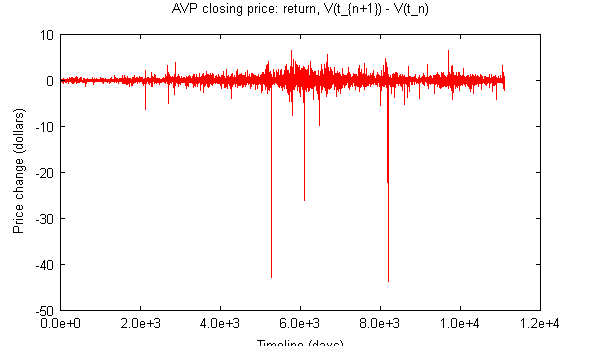
\includegraphics[scale=0.8]{figures/avp-price-close-diff.png}
\caption{Example time-series of the daily difference in closing price
of AVP stock.}
\label{fig:avp-price-diff}
\end{figure}

The underlying purpose in choosing such a model is to allow 
the change $d_n$ in asset value
to be regarded as being generated from a process, typically random,
 that may be separately modelled independently of the asset value history.
However, there are two problems with this additive model. 
Firstly, the value of $d_n$ is not independent of $V(t_{n})$,
since $V(t_{n+1})\ge 0$ implies that $d_n\ge -V(t_{n})$.
Secondly, $d_n$ is not
dimensionless, but has the same units as $V(t)$. Thus, sampling the
asset value in a difference currency would alter the analysis.

An alternative model that addresses both of these issues is the
multiplicative model:
\begin{eqnarray}
V(t_{n+1})  & = & V(t_{n}) (1+s_n)\,,
\label{eq:rate-of-return}
\end{eqnarray}
where, from equation~(\ref{eq:simple-additive}), we let
$s_n=V'(\xi_n)\delta t/V(t_{n})$, such that
$s_n$ is dimensionless.
Observe that $V(t_{n+1})\ge 0$ implies that
$s_n\ge -1$, so that $s_n$ is independent of $V(t_{n})$
(at least when regarded as a variable in its own right).
We define $s_n$ to be the {\em simple rate of return} over the
interval $t\in[t_{n},t_{n+1}]$, 
as shown in Figure~\ref{fig:avp-price-simple}.
\begin{figure}[hbt]
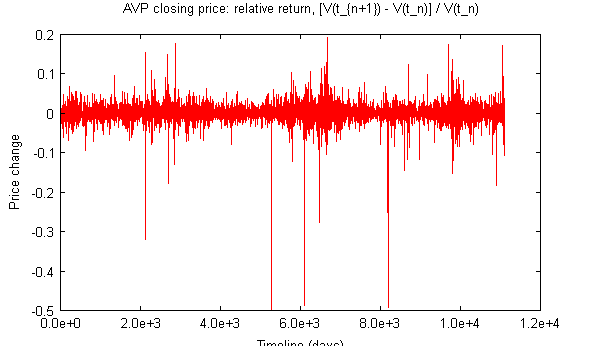
\includegraphics[scale=0.8]{figures/avp-price-close-simple.png}
\caption{Example time-series of the simple daily rate of return of
the closing price of AVP stock.}
\label{fig:avp-price-simple}
\end{figure}

This model has its uses when considering the total, relative change
in asset value over a period of time.
However, the values of $s_n$ are sometimes difficult to interpret, since they are not symmetrical about the origin. For example,
although $s_n=0$ implies no change in asset value, and $s_n=1$ implies a
doubling of asset value, the halving of asset value is implied by
$s_n=-\frac{1}{2}$ not $s_n=-1$.
In addition, the restriction that $s_n\in[-1,\infty)$ 
prevents us from modelling
$s_n$ as a random variable from common probability distributions that
have an unrestricted domain, especially the Gaussian, or Normal, distribution.

In order to handle this latter objection, we observe that
$V(t)\in[0,\infty)$ implies that $\ln V(t)\in(-\infty,\infty)$.
Hence, following along the lines of equation~(\ref{eq:Taylor-V}),
we turn to a Taylor series expansion
of $\ln V(t)$ around time $t=t_{n}$, to obtain
\begin{eqnarray}
\hspace*{-6mm}
\ln V(t_{n+1}) & = & \ln V(t_{n})+\frac{V'(t_{n})}{V(t_n)}\delta t
+\left[\frac{V''(t_{n})}{V(t_n)}
-\frac{V'(t_n)^2}{V(t_n)^2}\right]
\frac{(\delta t)^2}{2}
+\cdots\,.
\label{eq:Taylor-log-V}
\end{eqnarray}
This in turn (again via the Mean Value Theorem)
reduces to the log-additive model
\begin{eqnarray}
\ln V(t_{n+1}) & = & \ln V(t_{n})+r_n\,,
\label{eq:log-rate-of-return}
\end{eqnarray}
where $r_n=V'(\xi_n)\delta t/V(\xi_n)$ for some
$\xi_n\in[t_n,t_{n+1}]$. Note that $r_n$ differs
slightly from the definition of $s_n$ in the use of
$V(\xi_n)$ rather than $V(t_n)$ as the denominator.

After exponentiating boths side of equation~(\ref{eq:log-rate-of-return}), 
we obtain the alternative multiplicative form
\begin{eqnarray}
V(t_{n+1})  & =  & V(t_{n}) \;e^{r_n}\,.
\end{eqnarray}
Observe that $V(t_{n+1})\ge 0$ and $V(t_n)\ge 0$ together
imply that $r_n\in(-\infty,\infty)$.
We define $r_n$ to be the {\em logarithmic},
or {\em continuously compounded}, {\em rate of return} over
the interval $t\in[t_{n},t_{n+1}]$, due to the fact that
\begin{eqnarray}
\lim_{N\rightarrow\infty}\left(1+\frac{r_n}{N}\right)^{N} & = &
e^{r_n}\,.
\end{eqnarray}
Example values of $r_n$ are
show in Figure~\ref{fig:avp-price-log}.
\begin{figure}[hbt]
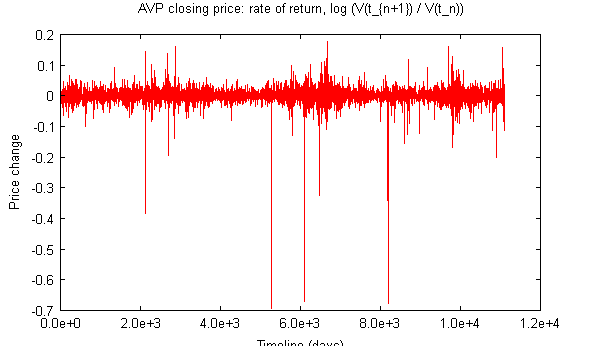
\includegraphics[scale=0.8]{figures/avp-price-close-log.png}
\caption{Example time-series of the logarithmic daily rate of return of
the closing price of AVP stock.}
\label{fig:avp-price-log}
\end{figure}

\end{document}
